\section{Simulation Analysis}
\label{sec:simulation}

The main circuit used to simulate the output impedance of the amplifier as a whole was the one that can be found in the following figure (repeteated from the analysis section).

\begin{figure}[h] \centering
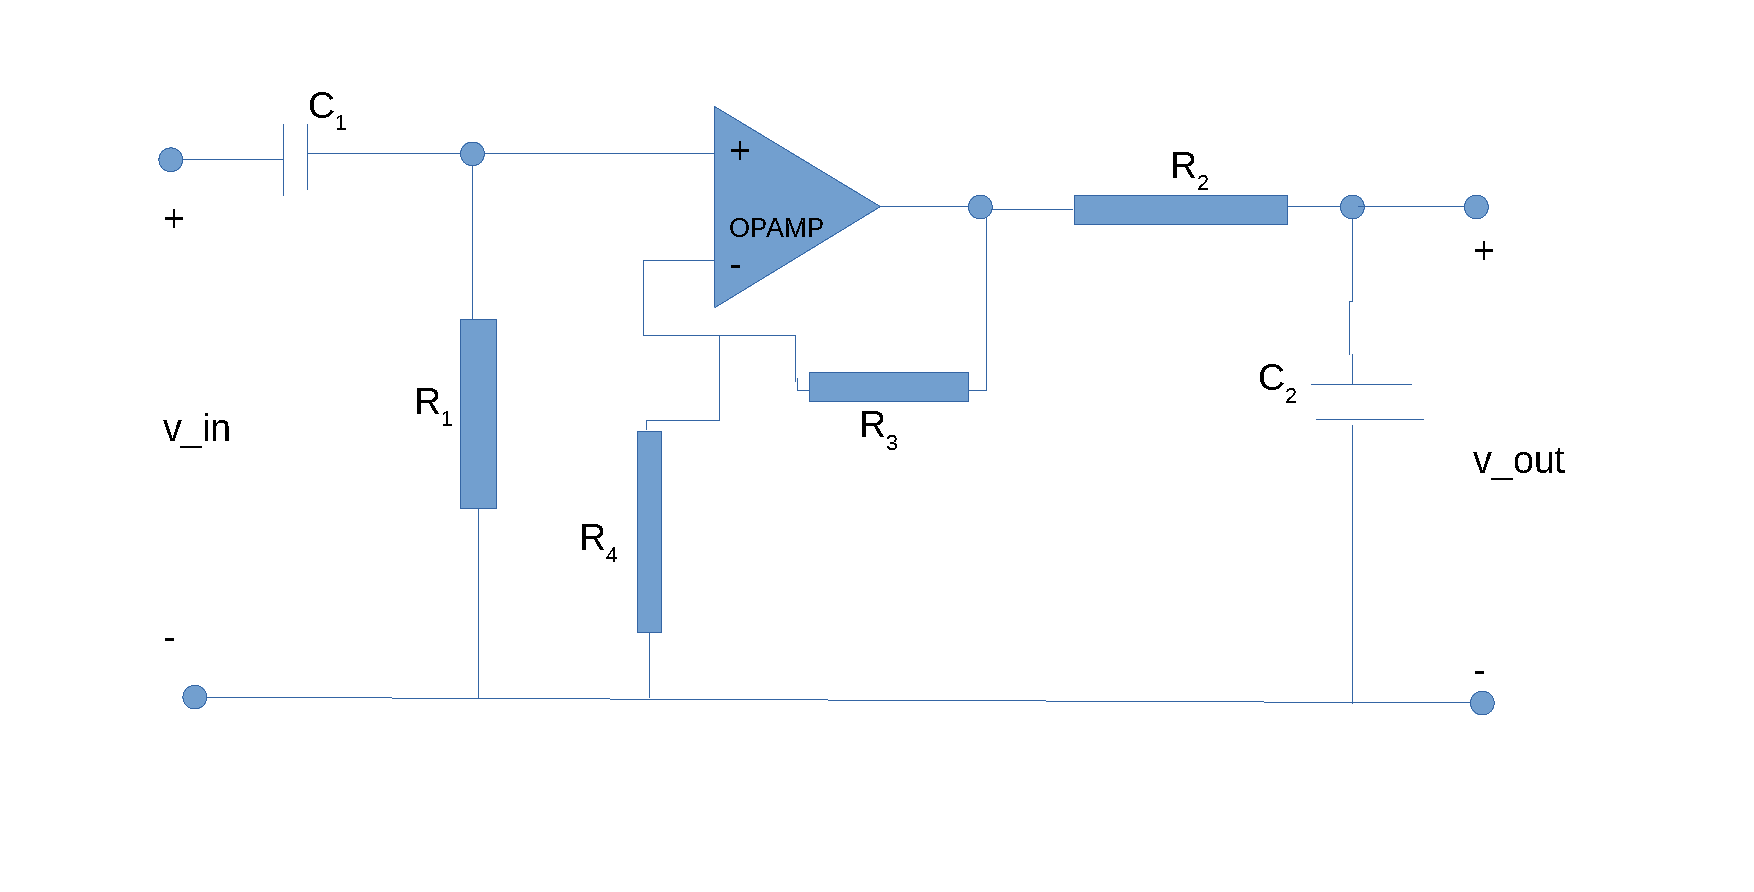
\includegraphics[width=0.95\linewidth]{diagram_t5.pdf}
%\vspace{-7cm}
\caption{Diagram of the circuit considered for the computations and simulations.}
\label{fig:diagram_t5_2}
\end{figure}


Initially, we began by translating this circuit to the Ngspice language, and ensuring the simulation was running smoothly, with random values for the parameters. Next, we automated the merit computation, and ensured all the correct plots were being adequately printed. Only then did we use the formulas referred to in the previous section, to try to work out a solution that gave us the desired pass band (at 1kHz), as well as the desired (40dB) gain. However, this was relatively easy, as the presential lab sesson had been quite informative and there we had already arrived at a setup that seemed to ensure us, approximately, the desired results. More on this in the following section.

However, we soon realized that the theoretical model we were based on was quite far from the simulation results... Having read up on the online class forum and thought about the problem at hand, we realized that this was mainly due to the way we were calculating the cutoff frequencies and the fact that the OPAMP model used was way more complex: besides being far from the ideal OPAMP model considered in our computations, the presence of capacitors (and not insignificant ones, at that!) had an impact on these same cutoff frequencies. As the objective all along was to maximize the Ngspice merit, and not the theoretical one, we focussed on improving this figure. This led us to opting for what might seem like strange combinations, that would never work on paper, but that did in practice. This process was quite iterative, due to a solid grasp on the concept of cutoff frquencies and how they should be altered by the variation of the corresponding resistor or capacitor, we managed to achieve a relatively central frquency at 1kHz. The gain was easier to fine-tune, with a relatively simple expression $1+\frac{R_3}{R_4}$ (this is just the gain from the OPAMP, not yet affected by the voltage drop across the input and output filters); here the limiting factor really was the limitation in terms of available resistors.

In the next table we reproduce the results for the final setup we settled on, already listed in the previous section, though hopefully here seen in new light. Do note that despite the available resistors being limited in quantity and value (only three of each of these types: 1$k\Omega$, 10$k\Omega$ and 100$k\Omega$), we were able to, combining these in parallels and in series, obtain a larger array of available equivalent resistor values: for example, with these nine resistors, we managed a 5$k\Omega$ resistor, a 150$k\Omega$ resistor, and a 1.5$k\Omega$ resistor (using, respectively, two 10$k\Omega$ resistors in parallel, three 100$k\Omega$ resistors, two in a parallel in series with the third, and an identical setup as the last, but with 1$k\Omega$ resistors instead of 100$k\Omega$ ones).


\hfill
 \parbox{1\linewidth}{
  \centering
  \begin{tabular}{|l|l|r|}
    \hline    
    {\bf Parameter} & {\bf Value} & {\bf Units }\\ \hline
    \input{values.tex}
  \label{tab:params2}
  \end{tabular}
  }
\par

\hfill
 \parbox{1\linewidth}{
  \centering
  \begin{tabular}{|l|l|l|r|}
    \hline    
    {\bf Parameter} & {\bf Simulation} & {\bf Theoretical } & {\bf Units }\\ \hline
    Zi & 766.402 & 640.49 & Ohm\\ \hline
Zo & 4.49605 & 2.9364 & Ohm\\ \hline
Cost & 8116 & Cost & MU\\ \hline
uco & 3106933.000 & 2123123123123.000 & Hz\\ \hline
lco & 7.924 & 2123123123123.000 & Hz\\ \hline
Bandwidth & 3106925.076 & 2123123123123.000 & Hz\\ \hline
Gainv(out) & 56.041 & -107.220 & [adimensional]\\ \hline
MERIT & 2707.5316 & -104.2260 & gold medals\\ \hline

  \label{tab:results2}
  \end{tabular}
  }
  
  For a more complete overview and comparison of the results, refer back to the previous section, where this discussion has been drawn out in quite some detail.

  
Next we present a number of plots, obtained from the Ngspice simulation, that help to illustrate the circuit's behaviour. Note in particular how the difference to the theoretical gain is here quite evident, and in particular how the phase bode plot is completely different.
  
\par
\vspace{-4cm}
\begin{figure}[H] \centering
\includegraphics[width=0.6\linewidth]{vdb_out.pdf}
\vspace{-1cm}
\caption{Output voltage gain frequency response - note the 40 dB gain in the passband.}
\label{fig:gain_sim}
\end{figure}


\begin{figure}[H] \centering
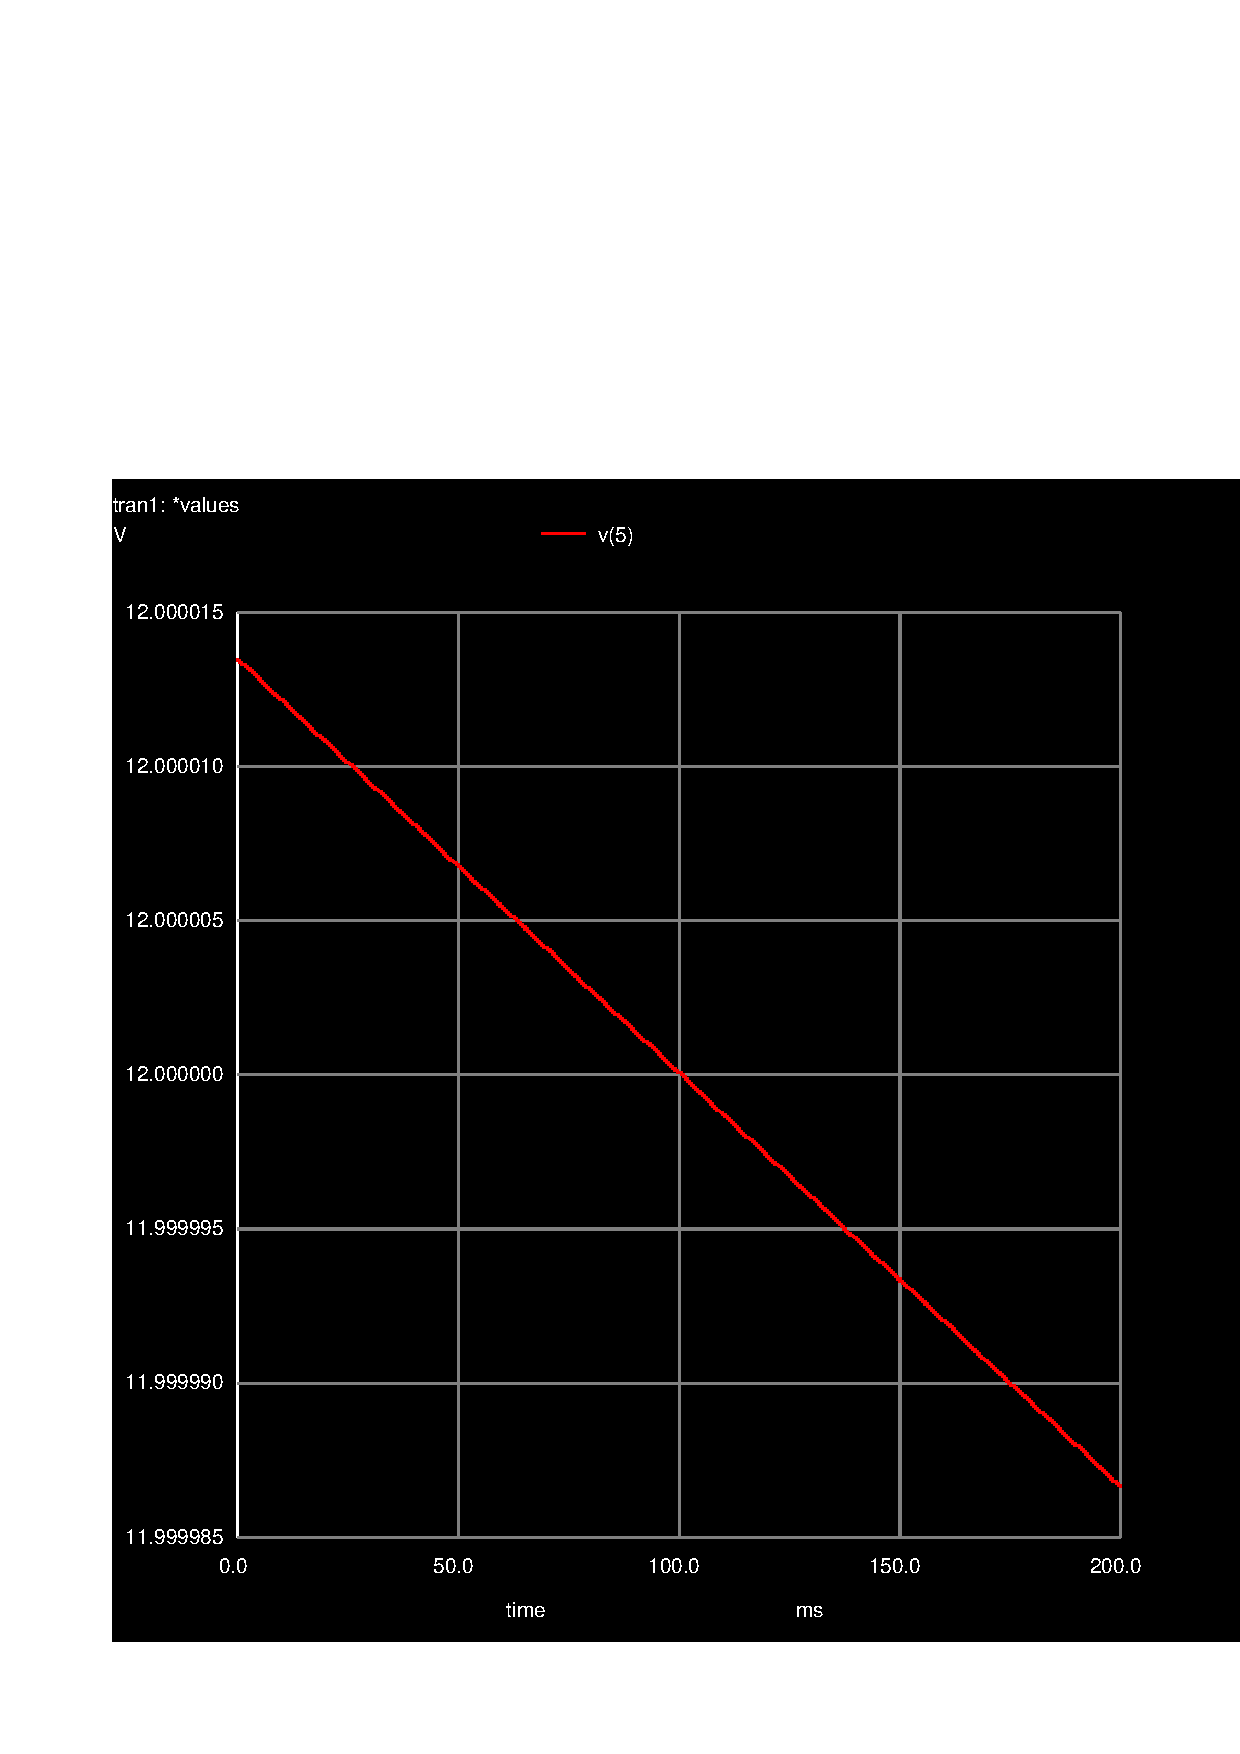
\includegraphics[width=0.5\linewidth]{vout.pdf}
\caption{The input and output signals, superimposed. The sheer scale of the amplification is evident here (the input, given the linear scale, is nearly a straight line with but only little ondulation around zero). The y axis is in V. Note that this graph is for the transient analysis, for which the voltage source only puts out 10mV, that with a gain of around $10^{2}$ goes to somewhere around 1V.}
\label{fig:In_imp}
\end{figure}
\vspace{-3cm}


\begin{figure}[H] \centering
\includegraphics[width=0.5\linewidth]{vp_out.pdf}
\caption{Phase bode plot of the circuit. Note how the plot decreases from plus 90 degrees down to zero, followed by a full 180 degree drop and finally another 90 degree drop, back to the initial plus 90 degrees phase. This indicates the existence of an additional two poles in the OPAMP model, not present in the ideal model we used for the theory section. If you remember the theoretical bode plot we obtained from octave, it is completely different! Note also that there is no discontinuity in this plot, it is just the way Ngspice presents the output of the arg() funtion, in the domain -180 degrees to 180 degrees.}
\label{fig:out_imp}
\end{figure}
\vspace{-3cm}


\pagebreak
